\subsection{Conceptual Description}
\label{sub:approach_conceptual_description}

\textbf{Architecture.} Figure~\ref{fig:stack} shows the \APIName stack.
On the bottom layer are the \textit{Application layer protocols}.
The Zeroconf protocols \textit{mDNS} and \textit{DNS-SD} are used for the advertisement and discovery of \APIshort services in the local network\footnote{We do not use these protocols directly but rely on their implementation in \textit{FlyWeb}.}. 
In terms of application-level network communication we use the common protocols of \textit{WebSocket} and \textit{HTTP}. 
The initial request to a \APIshort app is in form of a \textit{HTTP GET} request and associated requests for static resources.  Clients then establish a stable \textit{WebSocket} channel that is used for further communication between nodes (e.g. state replication). 
Above the application layer protocols is the \textit{FlyWeb} layer. 
We use FlyWeb as a library for facilitating interaction with the Zeroconf protocols. 
\APIName was designed with as few connection points with FlyWeb as possible such that this dependency can be easily replaced with a different implementation in the future. 
Above the FlyWeb layer is the \textit{\APIName} framework that exposes the API described in section~\ref{sub:approach_api_overview} to its applications that are located in the topmost layer.

\begin{figure}[h]
    \centering
    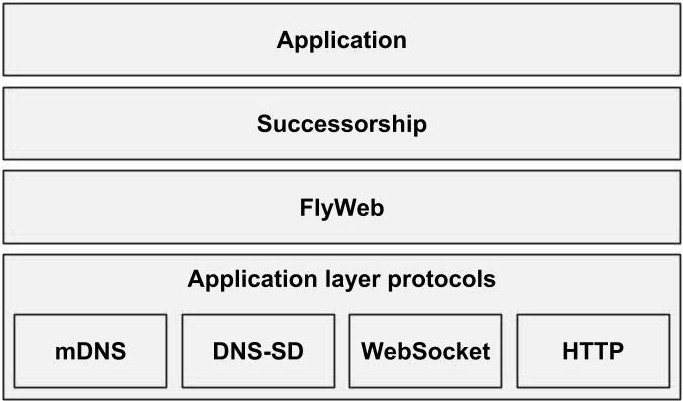
\includegraphics[width=\linewidth]{stack}
    \caption{Successorships Stack}
    \label{fig:stack}
\end{figure}

\noindent\textbf{Roles and shared state.} When a Shippy app is loaded in the browser the new node becomes either a client or server node. If it becomes a server node, it becomes a client node to ``itself'' shortly after. The application's global state is replicated and shared among all client nodes (see later paragraphs in this section for details). The global state can contain arbitrary application data and global metadata accessible only by the \APIshort library. One such required metadata field is a {\ttfamily successors} list containing a list of current clients, except the client node that is currently also the server. This list is used to determine which node should become the next server node upon failure of the current one. Figure~\ref{fig:roles} visualizes the distribution of roles. Node \textit{A} is currently the server with nodes \textit{B...n} being clients. The list of successors is shared in the global state accessible by all nodes.

\begin{figure}[h]
    \centering
    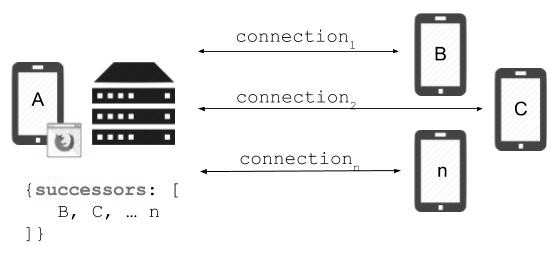
\includegraphics[width=\linewidth]{roles}
    \caption{Successorships Roles}
    \label{fig:roles}
\end{figure}

\noindent\textbf{Service discovery.} 
The \APIshort library described in section~\ref{sec:sub:approach_api_overview} comes with a compulsory Firefox add-on responsible for notifying apps with the current set of available \APIshort services. 
In the add-on, we register an event listener at a FlyWeb component {\ttfamily FlyWebDiscoveryManager} which is only available in the permission context of add-ons, making this a required mediator between FlyWeb and \APIshort Web apps. 
The {\ttfamily FlyWebDiscoveryManager} module dispatches a list of current local services in frequent intervals using the \textit{DNS-SD} protocol described in section~\ref{sub:background_zeroconf_networking}.
We sample these events to a maximum frequency of 100ms\footnote{We observed many duplicate and overly frequent event triggers from the {\ttfamily FlyWebDiscoveryManager} making this sampling necessary.} and filter out all services that were not published in the FlyWeb context\footnote{We aim to filter this list to contain only services published with Shippy rather than FlyWeb in the future, as described in section~\ref{sec:limitations_and_future_work}.}. We then dispatch our own events containing the current list of FlyWeb services with the service name, IP address and port on the Browser's global {\ttfamily window} object. 
These events are then accessible by any \APIshort app by registering an event listener as shown in listing~\ref{lst:service_discovery}.

\begin{lstlisting}[caption={Event listener for service discovery},label={lst:service_discovery}]
window.addEventListener('flywebServicesChanged', function(event) {
    let services = event.detail.services;
    // e.g. [{ serviceName: "QueueApp",
    // serviceUrl: "http://206.12.69.249:51629" }]
});
\end{lstlisting}

\noindent\textbf{Service publication.}

\noindent\textbf{Client succession.}

\noindent\textbf{State replication.}

\noindent\textbf{Handled fault scenarios.}

%Client Succession
%State Replication

% LIMITATIONS:
% all services are published to web apps
% ip + port => no hostnames
% only mac
% time to recovery
% weak consistency